\chapter{Methodology}
\label{cha:methodology}

\subsection{Work schedule}
\label{cha:work-schedule}



\begin{table}[h]
\resizebox{\textwidth}{!}{%
\begin{tabular}{|l|l|l|}
\hline
\multicolumn{1}{|c|}{\textbf{Week}} & \multicolumn{1}{c|}{\textbf{Goal}} \\ \hline
\begin{tabular}[c]{@{}l@{}}1-5\end{tabular} & \begin{tabular}[c]{@{}l@{}}- Topic identification \\ - Data sources analysis \\ 
 - Prototyping, tech stack exploration\end{tabular} \\ \hline
 \begin{tabular}[c]{@{}l@{}}6-7\end{tabular} & \begin{tabular}[c]{@{}l@{}}- Present a possible graph model and research statements \\ - Gather feedback, discuss and extend graph model, shape research statements\end{tabular} \\ \hline
 \begin{tabular}[c]{@{}l@{}}8-9\end{tabular} & \begin{tabular}[c]{@{}l@{}}- Working with a dataset \\ - Finalize tech stack \\ 
 - Visualisations\end{tabular} \\ \hline
 \begin{tabular}[c]{@{}l@{}}10-13\end{tabular} & \begin{tabular}[c]{@{}l@{}}- Implementation\end{tabular} \\ \hline
  \begin{tabular}[c]{@{}l@{}}13-15\end{tabular} & \begin{tabular}[c]{@{}l@{}}- Testing \\ - Documentation \\ 
 - Presentation\end{tabular} \\ \hline
\end{tabular}%
}
\caption{Work schedule for the research }
\label{table:work-schedule-research}
\end{table}

\subsection{Data acquisition}
\label{cha:data-acquisition}
In order to validate the hypotheses mentioned in the problem statement chapter of this paper, several possible data sources were explored. 
Because news articles are usually presented as unstructured data (no relationships), we also had to take into account the requirement of storing and exploring the data in a form of a graph.\\
\\
\noindent The following APIs were analysed and explored: \\

\begin{itemize}
\item[-] \url{https://newsapi.org/} - this api provides news articles and blog posts on various topics. It does not contain sentiments, and it is rate limited to 100 articles per day.
\item[-] \url{https://polygon.io/} - this api provides news articles on stock movements. It does not contain sentiments.
\item[-] \url{https://www.alphavantage.co/} - this api provides necessary data, including news articles, stock price data, as well as sentiments. The api access is rate limited, but still accessible for the purpose of this research.
\end{itemize}

\noindent We chose to use Alpha Vantage API, as it provides necessary data, which can be requested in JSON format using network calls written in any programming language.

\subsection{Data exploration}
\label{cha:data-exploration}
In order to explore the data the initial algorithm was written to access the data using breadth-first-search.
The example of news article contents:

\begin{lstlisting}[caption=Example of news article contents, captionpos=b, language=bash, label={lst:example-news-article-contents}]
{
           "title": "COP27 wins and losses: U.S. on the hook to pay for its pollution; natural gas gets nod as transition fuel",
           "url": "https://www.marketwatch.com/story/cop27-wins-and-losses-u-s-on
                   -the-hook-to-pay-for-its-pollution-natural-gas-gets-nod-as
                   -transition-fuel-11668964530",
           "time_published": "20221120T213700",
           "summary": "For the first time, rich nations, including top-polluting U.S., will pay for climate change damage inflicted on poorer nations. 'Developing' China can opt out."
"ticker_sentiment": [
               {
                   "ticker": "AAPL",
                   "relevance_score": "0.051276",
                   "ticker_sentiment_score": "-0.137418",
                   "ticker_sentiment_label": "Neutral"
               },
]
...
}
\end{lstlisting}


\noindent Each article contains a list (ticker\_sentiment), which lists tickers of the companies mentioned in the article, with the sentiment score and label attached. This allows us to use this ticker information to get information about the company, such as an industry sector the company belongs to.

\noindent The article information also has a date, on which it was published, which we can use to request a range of stock prices (daily open and close prices). Using these prices we can determine if the sentiments of the news article have a correlation with stock price movements.

\noindent We also can use the ticker to request news articles about companies mentioned in the already visited article.
\\
\\
\noindent As we discovered, when traversing over the data in this way, we can build an initial graph (as an adjacency list) to see if it can be valid for our research (if there are relationships between nodes).



\begin{figure}[h]
 \centering
 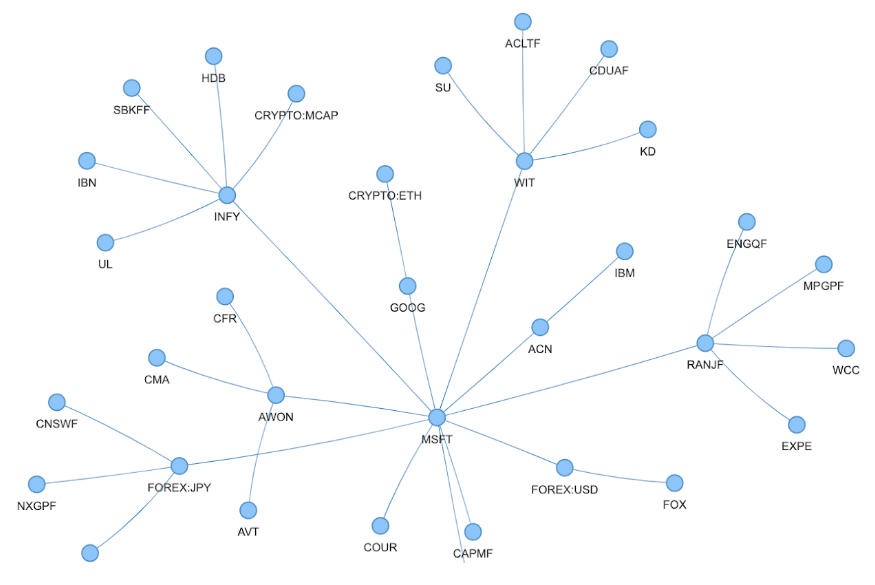
\includegraphics[width=0.8\textwidth]{images/nodes-representation-graph.png}
 \caption{Representation of the nodes in a graph }
 \label{fig:nodes-representation-as-graph}
\end{figure}



As we can see in the figure \ref{fig:nodes-representation-as-graph}, the nodes can be represented as companies, and relationships can be represented as ``being mentioned in the same news article``. This gives us an overview of the data and confirms the possibility of graph structure for the news coverage.



\subsection{Data preparation}
\label{cha:data-preparation}
The data is processed in the following ways:

\begin{itemize}
\item[-] the numeric values, such as stock price or sentiment values are represented as floats to make search queries easier for the database;
\item[-] the date values are converted to DateTime objects to facilitate date calculations and search queries;
\item[-] the information about other types of securities, such as currencies or cryptocurrencies, is excluded;
\item[-]the duplicated news articles and companies are excluded;
\item[-] duplicate keys for possible nodes (news article, company, etc.) are excluded or renamed.
\end{itemize}








